
\section{Design Iteration 2}
\label{sec: design iteration 2 captive}
The first design iteration is suitable to map the response surfaces over a wide spectrum of input factors and thus determine the rough location of the optima. But due to the wide variety of the data points, the reliability of the output optima is limited. However, this can be increased by doing a second design iteration, where a new design space is made with a narrower design spectrum, where the parameter boundaries are less spread and lie around the optima.

\subsection{Approach}
Based on the results of the first design iteration, the boundaries for the second design iteration are established and shown in Table \ref{tab: boundaries DI2 captive}. The complete design space, including results, is shown in Table \ref{tab: params design iteration 2 captive setup} Appendix \ref{app: parameters configurationss}.

\begin{table}[h]
\centering
\scalebox{0.65}{
\begin{tabular}{@{}ccccc@{}}
\toprule
Factor & Name        & Units        & Minimum & Maximum       \\ \midrule
A & T               & m & 9.50   & 12.50   \\
B & W               & m & 120.00  & 150.00   \\
C & front\_fraction & - & 0.010 & 0.99  \\
D & top\_fraction   & - & 0.010 & 0.99  \\
E & radius          & m & 1500.00 & 2000.00 \\
F & WL              & m & 0.50  & 2.50     \\ \bottomrule
\end{tabular}
}
\caption{Boundaries Design Space Captive Design Iteration 2}
\label{tab: boundaries DI2 captive}
\end{table}

\subsection{Performance breakwaters}
\label{sec: DI1 captive H3 performance bw}

The performance of the breakwater in terms of minimising the mean wave drift force and maximising wave attenuation is shown in Figure \ref{fig: Fd vs. Kt DI2 H3 captive}, from which it can be seen that now more breakwaters are indeed performing better in both phenomena, compared to the first design iteration. The Pareto front obviously consists of more breakwaters. Some of them have a geometry shown in Figure \ref{fig: pareto front bw DI2 H3 captive}. Again, large box-type structures around the waterline are best at attenuating wave energy, and those containing a sloping beach on their wave-ward side are good at minimising the mean wave drift force. 


\begin{figure}[h]
    \centering
    \begin{subfigure}[b]{0.49\textwidth}
        \centering
        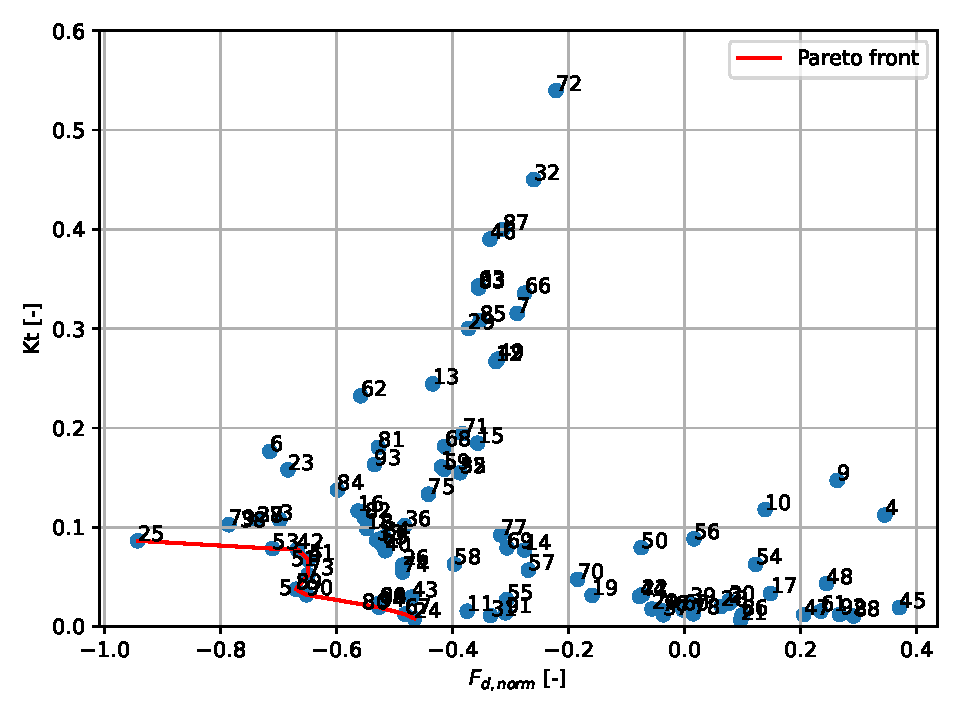
\includegraphics[width=\linewidth]{figures/ComFLOW/Results DI2/Fd_norm_VS_Kt_normal.pdf}
        \caption[]%
        {{\small All breakwaters}}    
        \label{fig: Fd vs. Kt DI2 H3 captive normal}
    \end{subfigure}
    \hfill
    \begin{subfigure}[b]{0.49\textwidth}  
        \centering 
        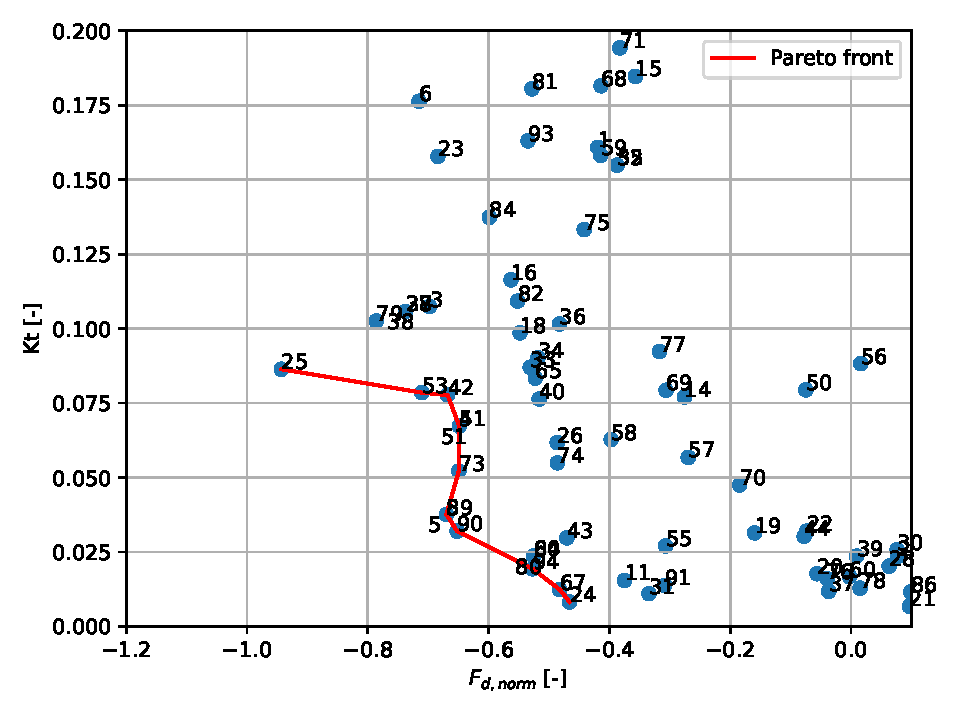
\includegraphics[width=\linewidth]{figures/ComFLOW/Results DI2/Fd_norm_VS_Kt_Pareto.pdf}
        \caption[]%
        {{\small Pareto front}}    
        \label{fig: Fd vs. Kt DI2 H3 captive pareto}
    \end{subfigure}
    
    \caption{Mean wave drift force vs. Wave transmission}
    \label{fig: Fd vs. Kt DI2 H3 captive}
\end{figure}



\begin{figure}[h]
    \centering
    \begin{subfigure}[b]{0.49\textwidth}
        \centering
        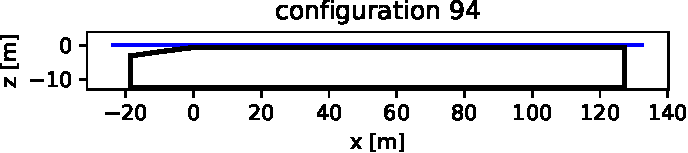
\includegraphics[width=\linewidth]{figures/ComFLOW/Breakwater Geometries/Design Iteration 2 captive/breakwater_geometry94.pdf}
        \caption[]%
        {{\small }}    
        \label{}
    \end{subfigure}
    \hfill
    \begin{subfigure}[b]{0.49\textwidth}  
        \centering 
        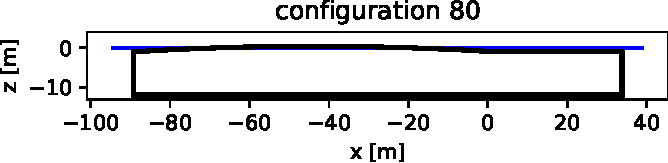
\includegraphics[width=\linewidth]{figures/ComFLOW/Breakwater Geometries/Design Iteration 2 captive/breakwater_geometry80.pdf}    
        {{\small }}    
        \label{}
    \end{subfigure}
    
    \centering
    \begin{subfigure}[b]{0.49\textwidth}
        \centering
        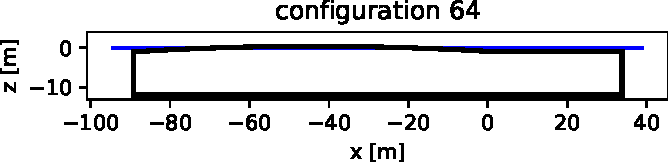
\includegraphics[width=\linewidth]{figures/ComFLOW/Breakwater Geometries/Design Iteration 2 captive/breakwater_geometry64.pdf}    
        \caption[]%
        {{\small }}    
        \label{}
    \end{subfigure}
    \hfill
    \begin{subfigure}[b]{0.49\textwidth}  
        \centering 
        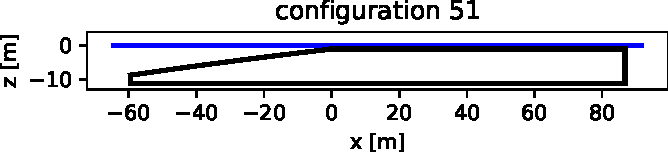
\includegraphics[width=\linewidth]{figures/ComFLOW/Breakwater Geometries/Design Iteration 2 captive/breakwater_geometry51.pdf}    
        \caption[]%
        {{\small }}    
        \label{}
    \end{subfigure}
    
    \centering
    \begin{subfigure}[b]{0.49\textwidth}
        \centering
        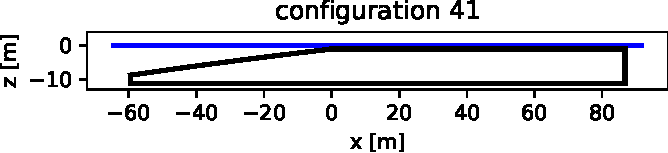
\includegraphics[width=\linewidth]{figures/ComFLOW/Breakwater Geometries/Design Iteration 2 captive/breakwater_geometry41.pdf}    
        \caption[]%
        {{\small }}    
        \label{}
    \end{subfigure}
    \hfill
    \begin{subfigure}[b]{0.49\textwidth}  
        \centering 
        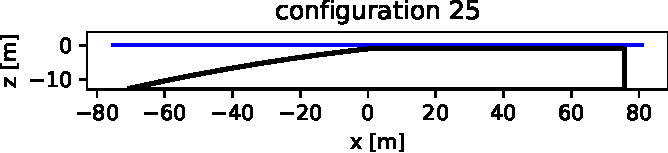
\includegraphics[width=\linewidth]{figures/ComFLOW/Breakwater Geometries/Design Iteration 2 captive/breakwater_geometry25.pdf}    
        \caption[]%
        {{\small }}    
        \label{}
    \end{subfigure}
    
    \caption{Wave breakers on Pareto front}
    \label{fig: pareto front bw DI2 H3 captive}
\end{figure}





\subsection{Design Optima}
Based on the data found by ComFLOW, the response surfaces were plotted from which the design optima are found and presented in this section. 


\subsubsection{Based on minimal mean wave drift force}
Again, the first six optima based on a minimal mean wave drift force converged to the lowest value of $T$. Therefore, the structure is placed slightly closer to the waterline, which is consistent with the response surface of Figure \ref{fig: Fd_T_WL_wedge DI1 H3 captive}. In addition, these optima converged to the lowest width $W$. All the top fractions of configurations 1 to 6 are 0.99, so they are box-type structures. 
The last four optima are larger structures, placed closer to the water surface and possess a sloping beach. Configurations 1 and 7 experienced the same mean wave drift force, but Configuration 1 has better wave attenuation performances. 


\begin{table}[h]
\centering
\scalebox{0.65}{
\begin{tabular}{@{}ccccccccccc@{}}
\toprule
configuration & T        & W        & front\_fraction & top\_fraction & radius   & WL & $F_{d,norm,DoE}$ & $K_{t,DoE}^2$  & $F_{d,norm,ComFLOW}$  & $K_{t,ComFLOW}^2$      \\ \midrule
1  & 9.50  & 120.00 & 0.59 & 0.99 & 1500.00 & 2.16 & -0.96 & 0.009  & -0.51 & 0.043\\
2  & 9.52  & 120.00 & 0.58 & 0.99 & 1500.00 & 2.17 & -0.95 & 0.009  \\
3  & 9.51  & 121.03 & 0.58 & 0.99 & 1500.04 & 2.14 & -0.95 & 0.008  \\
4  & 9.50  & 126.18 & 0.58 & 0.99 & 1500.00 & 2.06 & -0.94 & 0.005  \\
5  & 9.50  & 120.00 & 0.52 & 0.97 & 1500.00 & 2.24 & -0.94 & 0.010  \\
6  & 9.50  & 122.12 & 0.47 & 0.99 & 1502.39 & 1.92 & -0.94 & 0.005  \\
7  & 12.11 & 150.00 & 0.010 & 0.66 & 1519.49 & 0.89 & -0.94 & -0.002 &-0.51 & 0.080 \\
8  & 12.21 & 150.00 & 0.010 & 0.64 & 1542.35 & 0.79 & -0.93 & -0.002 \\
9  & 12.08 & 149.97 & 0.010 & 0.68 & 1543.32 & 0.92 & -0.93 & -0.001 \\
10 & 12.18 & 150.00 & 0.010 & 0.62 & 1508.26 & 0.82 & -0.93 & -0.002 \\ \bottomrule


\end{tabular}
}
\caption{Parameters optimal breakwaters based on minimal mean wave drift force}
\label{tab: most optimal breakwaters DI2 Fd}
\end{table}


\begin{figure}[h]
    \centering
    \begin{subfigure}[b]{0.475\textwidth}
        \centering
        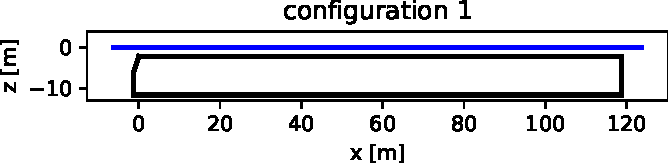
\includegraphics[width=\textwidth]{figures/ComFLOW/Breakwater Geometries/Design Iteration 2 captive/breakwater_geometry1_Fd.pdf}
        \caption[]%
        {{\small}}    
        \label{fig: opt breakwater 1 DI2}
    \end{subfigure}
    \hfill
    \begin{subfigure}[b]{0.475\textwidth}
        \centering
        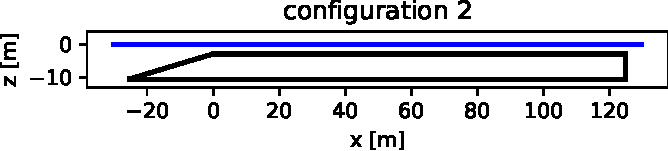
\includegraphics[width=\textwidth]{figures/ComFLOW/Breakwater Geometries/Design Iteration 2 captive/breakwater_geometry2_Fd.pdf}
        \caption[]%
        {{\small}}    
        \label{fig: opt breakwater 1 DI2}
    \end{subfigure}
    \caption{The most optimal breakwaters based on mean wave drift force}
    \label{fig:  most optimal breakwaters DI2}
\end{figure}









\subsubsection{Based on minimal transmission coefficient}
Most of the design optima converged to a depth $T$ within the parameter limits. Interesting is that for wave transmission performance, the breakwaters did not converge to the largest width $W$. The biggest difference in comparison with the first six optima based on a minimal mean wave drift force (previous section) is that the breakwaters are placed closer to the waterline and a large sloping beach is present. The optima are similar to optima 7 to 10 of previous section. All optima found also have a negative mean wave drift force. 



\begin{table}[h]
\centering
\scalebox{0.65}{
\begin{tabular}{@{}ccccccccccc@{}}
\toprule
configuration & T        & W        & front\_fraction & top\_fraction & radius   & WL & $F_{d,norm,DoE}$ & $K_{t,DoE}^2$  & $F_{d,norm,ComFLOW}$  & $K_{t,ComFLOW}^2$      \\ \midrule
1  & 11.42 & 138.22 & 0.11 & 0.46 & 1592.55 & 0.81 & -0.73 & -0.0010 & -0.73 & 0.014\\
2  & 10.13 & 120.00 & 0.57 & 0.51 & 1897.50 & 0.50 & -0.39 & -0.0020 \\
3  & 10.06 & 123.15 & 0.93 & 0.97 & 1572.39 & 0.95 & -0.56 & -0.0030 \\
4  & 10.21 & 145.03 & 0.089 & 0.71 & 1552.15 & 1.28 & -0.80 & -0.0010 \\
5  & 9.50  & 138.50 & 0.36 & 0.91 & 1971.47 & 2.40 & -0.67 & -0.00 \\
6  & 9.50  & 120.00 & 0.99 & 0.010 & 2000.00 & 0.50 & -0.65 & -0.0030 \\
7  & 9.68  & 140.51 & 0.66 & 0.35 & 1970.37 & 1.35 & -0.37 & -0.000 \\
8  & 11.51 & 136.72 & 0.37 & 0.49 & 1769.89 & 0.89 & -0.60 & -0.000 \\
9  & 11.17 & 147.83 & 0.78 & 0.55 & 1536.11 & 1.47 & -0.44 & -0.0010 \\
10 & 9.92  & 142.98 & 0.030 & 0.88 & 1572.12 & 1.46 & -0.80 & -0.0020 \\ \bottomrule


\end{tabular}
}
\caption{Parameters optimal breakwaters based on minimal transmission coefficient}
\label{tab: most optimal breakwaters DI2 Kt}
\end{table}


\begin{figure}[h]
    \centering
    \begin{subfigure}[b]{0.475\textwidth}
        \centering
        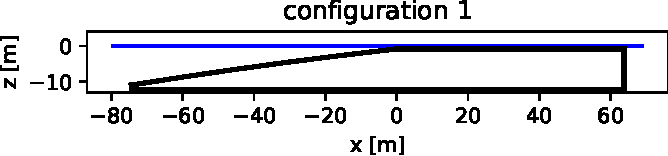
\includegraphics[width=\textwidth]{figures/ComFLOW/Breakwater Geometries/Design Iteration 2 captive/breakwater_geometry1_Kt.pdf}
        \caption[]%
        {{\small}}    
        \label{fig: opt breakwater 1 DI2}
    \end{subfigure}

    
    \caption{The most optimal breakwater based transmission coefficient}
    \label{fig:  most optimal breakwaters DI2}
\end{figure}















